% !TEX root = B&G_oefeningen.tex
\chapter{Binaire bomen}

\section*{Inleiding}


Je herkent de klassieke structuur met \verb+domain+ en \verb+ui+. Je zal vooral methodes toevoegen in het java bestand \verb=binaryTree= in \verb+domain+ en dan code uittesten in \verb+ui+.

Als je de broncode hebt geopened moet je  misschien nog aangeven dat de code in het mapje \verb+src+ de source is. Kies daarvoor in het menu \verb+File > project structure+ en duid bij het blad \verb+Modules+ de \verb+src+ map aan als \verb+Sources+. De Java bestanden krijgen nu als icoontje een blauwe cirkel met een letter ‘c’ er in.

We maken eerst twee oefeningen op bomen op papier (\papier). Vanaf oefening 2.3 schrijf je nieuwe methodes (\code).


\begin{oef}
\papier Bekijk de boom uit figuur~\ref{fig:binboom} op pagina~\pageref{fig:binboom}
\begin{figure}[htbp]
    \centering
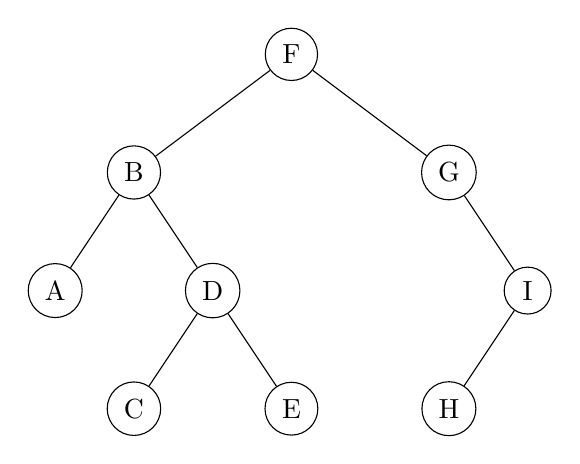
\begin{tikzpicture}[every node/.style={circle,draw},
				level 1/.style={sibling distance=40mm},
				level 2/.style={sibling distance=20mm}]
\node {F}
child { node {B} 
	child { node {A} }
	child { node {D} 
		child { node {C} } 
		child { node {E} } }
}
child { node {G}
	child[missing]
	child { node {I}
		child { node {H}}
		child[missing]}};
\end{tikzpicture}
\caption{Een (binaire?) boom}
    \label{fig:binboom}
\end{figure}

\begin{oefenumerate}[label=\alph*)]
	\item Is dit een binaire boom?
	\item Wat is de wortel van deze boom?
	\item Wat is de diepte van deze boom?
	\item Is deze boom compleet?
	\item Geef alle bladeren van deze boom.
	\item Geef alle interne knopen van deze boom.
	\item Hoeveel knopen bevat de linkersubboom? Teken deze subboom.
	\item Schrijf de knopen van de gegeven boom (zie fig.~\ref{fig:binboom}) op in de volgorde waarin ze bezocht worden bij een pre-order wandeling.
	\item Schrijf de knopen van de gegeven boom (zie fig.~\ref{fig:binboom}) op in de volgorde waarin ze bezocht worden bij een in-order wandeling.
	\item Schrijf de knopen van de gegeven boom (zie fig.~\ref{fig:binboom})op in de volgorde waarin ze bezocht worden bij een post-order wandeling.
\end{oefenumerate}
\begin{opl}

\begin{oefenumerate}
	\item Ja want elke knoop in deze boom heeft maximaal 2 kinderen.
	\item Knoop F.
	\item Het maximaal aantal knopen van een pad van de wortel naar 
een blad is vier, dus de diepte van deze boom is vier.
	\item Neen, niet compleet.
Alle niveaus behalve eventueel de laatste zijn niet 
volledig gevuld. Zo ontbreekt er een knoop op niveau 3: 
het linkerkind van knoop G. 
Verder zijn alle knopen op het laatste niveau ook niet 
aan de linkerzijde: de twee kinderen van knoop A ontbreken.
	\item Knopen A, C, E en H.
	\item Knopen F, B, D, G en I.
	\item Deze subboom bevat 5 knopen.
	\item F B A D C E G I H
	\item A B C D E F G H I
	\item A C E D B H I G F

	
\end{oefenumerate}
\end{opl}
\end{oef}


\begin{oef} 
\papier \code Voor deze oefening duiken we in de code die je in IntelliJ geïmporteerd hebt.
\begin{oefenumerate}
	\item Bestudeer de implementatie van \verb=BinaryTree<E>=. Stel vragen als er onduidelijkheden zijn.
	\item Bestudeer de \verb=main= functie in de \verb=BinaryTreeDriver= klasse. Hierin wordt een boom aangemaakt waarmee de functie \verb=printPreorder= wordt geïllustreerd. Deze functie is een recursieve implementatie om de waarden van de knopen in pre-order volgorde af te printen.
	\item Teken de boom uit de driver klasse op papier.
	\item Schrijf op papier de verwachte output bij het doorlopen van de boom in pre-order.
	\item Test je verwachte output door de diver-klasse te runnen.
	\item Vervang de code in de driver-klasse door de constructie van de boom uit oefening 2.1.
	\item Run de code en controleer op die manier je antwoord op vraag h) van oefening 2.1.
\end{oefenumerate}
\begin{opl}
\begin{oefenumerate}
\item
\item
\item Figuur~\ref{fig:binboomopgave} toont een grafische voorstelling van de gegeven boom.
\begin{figure}[htbp]
    \centering
\begin{tikzpicture}[every node/.style={},
				level 1/.style={sibling distance=40mm},
				level 2/.style={sibling distance=20mm},
				level 3/.style={sibling distance=10mm}]]
\node {C}
child { node {A} 
	child { node {D} }
	child { node {F} }
}
child { node {G}
	child {node {E}
		child { node {H}}
		child[missing]}
	child { node {B}}};		
\end{tikzpicture}
\caption{Boom uit oefening 2}
    \label{fig:binboomopgave}
\end{figure}
\item Een preorder doorloop geeft: C A D F G E H B.
\item
\item De code van de boom uit oefening 1 kan er als volgt uitzien:
\begin{lstlisting}[caption={Binaire boom uit oefening 1}, label=binoef1]
package ui;

import domain.BinaryTree;

public class BinaryTreeDriver2 {

	public static void main(String[] args) {
		//begin bij de bladeren ...
		BinaryTree<String> nodeA = new BinaryTree<>("A");
		BinaryTree<String> nodeC = new BinaryTree<>("C");
		BinaryTree<String> nodeE = new BinaryTree<>("E");
		BinaryTree<String> nodeH = new BinaryTree<>("H");

		// ... ga vervolgens naar alle interne knopen ...
		// knoop I heeft links H en rechts niets
		BinaryTree<String> nodeI = new BinaryTree<>("I",nodeH, null);
		// knoop G heeft links niets en rechts I
		BinaryTree<String> nodeG = new BinaryTree<>("G",null, nodeI);
		// knoop D heeft links C en rechts E
		BinaryTree<String> nodeD = new BinaryTree<>("D",nodeC,nodeE);
		// knoop B heeft links A en rechts D
		BinaryTree<String> nodeB = new BinaryTree<>("B",nodeA, nodeD);
		
		// ... en eindig met de wortel
		// boom heeft root F en heeft links B en rechts G
		BinaryTree<String> boom = new BinaryTree<>("F",nodeB, nodeG);
		boom.printPreorder();
	}

}
 \end{lstlisting}
 
 \item F B A D C E G I H 
\end{oefenumerate}

\end{opl}
\end{oef}




\begin{oef}
\code Van pre-order naar in-order …
\begin{oefenumerate}
	\item Implementeer volledig analoog aan \verb=printPreorder= een recursieve implementatie \verb=printInorder= om de waarden van de knopen in in-order volgorde af te printen.
	\item Controleer je implementatie met behulp van je testvoorbeeld. Ga ook na of de uitvoer overeenkomt met je antwoord op vraag i) van oefening 2.1.
\end{oefenumerate}
\begin{opl}
In het \verb+domain+ package voeg je in \verb+BinaryTree.java+ volgende methode in:
\begin{lstlisting}[caption={In-order doorloop van een binaire boom}, label=bininorder]
public void printInorder(){
	if (this.leftTree != null) {
		this.leftTree.printInorder();
	}
	System.out.print(this.data + " ");
	if (this.rightTree != null) {
		this.rightTree.printInorder();
	}
}
\end{lstlisting}

\end{opl}
\end{oef}


\begin{oef}
\code … en naar post-order.
\begin{oefenumerate}
	\item Implementeer volledig analoog aan \verb=printPreorder= en \verb=printInorder= een recursieve implementatie \verb=printPostorder= om de waarden van de knopen in post-order volgorde af te printen.
	\item Controleer je implementatie met behulp van je testvoorbeeld. Ga op die manier ook na of de uitvoer  overeenkomt met je antwoord op vraag j) van oefening 2.1.
\end{oefenumerate}
\begin{opl}
In het \verb+domain+ package voeg je in \verb+BinaryTree.java+ volgende methode in:
\begin{lstlisting}[caption={Post-order doorloop van een binaire boom}, label=binpostorder]
public void printPostorder(){
	if (this.leftTree != null) {
		this.leftTree.printPostorder();
	}
	if (this.rightTree != null) {
		this.rightTree.printPostorder();
	}
	System.out.print(this.data + " ");
}
\end{lstlisting}
\end{opl}
\end{oef}


\begin{oef}
\code Het doel van deze opdracht bestaat erin om een recursieve implementatie te schrijven voor het bepalen van het aantal knopen van een boom.

\begin{oefenumerate}
	\item Ga voor de boom uit oefening 2.1 na dat het aantal knopen kan gevonden worden als volgt:  1 + als er een linkersubboom is: het aantal knopen van de linkersubboom  + als er een rechtersubboom is: het aantal knopen van de rechterSubboom.
	\item Gebruik het vorige idee om een recursieve implementatie \verb=countNodes= te schrijven om het aantal knopen van een binaire boom te bepalen.
	\item Controleer je implementatie van \verb=countNodes= met behulp van je testvoorbeeld in de \verb=main= functie.
\end{oefenumerate}
\begin{opl}
Je vindt het correcte aantal knopen (9) bvb. met de methode \verb+countNodes+ die je implementeert in \verb+BinaryTree.java+. Vanzelfsprekend kan je met \verb+if+ constructies werken, maar de \emph{ternaire operator} van java maakt de code wel een stuk kernachtiger (listing~\ref{bincountnodes}).
\begin{lstlisting}[caption={Tel het aantal knopen in een binaire boom}, label=bincountnodes]
public int countNodes() {
	return 1 + (this.leftTree == null ? 0 : this.leftTree.countNodes())
					+ (this.rightTree == null ? 0 : this.rightTree.countNodes());
}
\end{lstlisting}
\end{opl}
\end{oef}


\begin{oef}
\code Schrijf een recursieve implementatie voor het bepalen van de diepte van een gegeven binaire boom. 
\begin{oefenumerate}
	\item Ga voor de boom uit oefening 1 na dat zijn diepte kan gevonden worden als 1 + het maximum van de diepte van de linker- en rechtersubboom van de boom.
	\item Gebruik het vorige idee om een recursieve implementatie \verb=getDepth= te schrijven om de diepte van een binaire boom te bepalen.
	\item Controleer je implementatie van \verb=getDepth= met behulp van je testvoorbeeld in de \verb=main= functie.
\end{oefenumerate}
\begin{opl}
Je vindt de maximale diepte van een boom met de methode \verb+getMaxDepth+ die je implementeert in \verb+BinaryTree.java+. Ook hier weer een oplossing met de \emph{ternaire operator} van java (listing~\ref{bingetmaxdepth}).
\begin{lstlisting}[caption={De diepte van een binaire boom}, label=bingetmaxdepth]
public int getDepth() {
	return 1 + Math.max((this.leftTree == null ? 0 : this.leftTree.getDepth()), 
					(this.rightTree == null ? 0 : this.rightTree.getDepth()));
}
\end{lstlisting}

\end{opl}
\end{oef}


\begin{oef}
\code Schrijf een functie \verb=isLeaf= om na te gaan of een boom een blad is. Dit wil zeggen dat de linkerdeelboom en de rechterdeelboom leeg zijn.
\begin{opl}
Listing~\ref{binisleaf} toont een eenvoudige implementatie voor deze functie.
\begin{lstlisting}[caption={Is een knoop een blad?}, label=binisleaf]
public boolean isLeaf() {
	return this.leftTree == null && this.rightTree == null;
}
\end{lstlisting}
\end{opl}
\end{oef}




\begin{oef}
\code Het doel van deze opdracht bestaat erin om een recursieve implementatie te schrijven voor het bepalen van het aantal bladeren van een boom.

\begin{oefenumerate}
	\item Ga voor de boom uit oefening 1 na dat het aantal bladeren kan gevonden worden als volgt:  1 voor een boom die enkel 1 blad bevat en anders de som van het aantal bladeren van de linkersubboom als er een linkersubboom is en het aantal bladeren van de rechtersubboom als  er een rechtersubboom is.
	\item Gebruik het vorige idee om een recursieve implementatie \verb=countLeaves= te schrijven om het aantal bladeren van een binaire boom te bepalen.
	\item Controleer je implementatie van \verb=countLeaves= met behulp van je testvoorbeeld in de \verb=main= functie.
\end{oefenumerate}
\begin{opl}
Listing~\ref{bincountleaves} toont een eenvoudige implementatie voor deze functie.
\begin{lstlisting}[caption={Hoeveel bladeren bevat deze boom?}, label=bincountleaves]
public int countLeaves() {
	if (this.isLeaf()) {
		return 1;
	} else {
		return (this.leftTree == null ? 0 : this.leftTree.countLeaves()) 
					+ (this.rightTree == null ? 0 : this.rightTree.countLeaves());
	}
}
\end{lstlisting}
\end{opl}
\end{oef}

\begin{oef}
\code In deze oefening schrijf je een recursieve implementatie \verb=getDataLeaves=  voor het bepalen van een lijst van datavelden van de bladeren van een boom. Controleer je implementatie met behulp van je testvoorbeeld en vergelijk de uitvoer met je antwoord op vraag e) uit oefening 2.1. De volgorde zal natuurlijk afhangen van het soort wandeling dat je gebruikt.
\begin{opl}
Deze methode is wat moeilijker dan de vorige omdat je nu met lijsten moet werken. Listing~\ref{bingetdataleaves} toont een mogelijke implementatie. Met een lus in de \verb+main+ methode kan je als test de data van alle bladeren uitschrijven.
\begin{lstlisting}[caption={Genereer een lijst met de data van alle bladeren}, label=bingetdataleaves]
public ArrayList<E> getDataLeaves() {
	ArrayList<E> res = new ArrayList<>();
	if (this.isLeaf()) {
		res.add(this.data);
	} else {
		res = (this.leftTree == null ? new ArrayList<>() : this.leftTree.getDataLeaves());
		ArrayList<E> rightLeaves = 
			(this.rightTree == null ? new ArrayList<>() : this.rightTree.getDataLeaves());
		res.addAll(rightLeaves);
	}
	return res;
}
\end{lstlisting}

\end{opl}
\end{oef}

\begin{oef}
\code Programmeer een recursieve implementatie voor het bepalen of een gegeven data-veld in de binaire boom voorkomt. Schrijf een methode \verb=contains= die gegeven een data-veld true teruggeeft indien de boom een knoop bevat met het gegeven data-veld en false anders. Probeer in je \verb+main+ deze functionaliteit uit door vier keer de functie op te roepen met respectievelijk “D”, “H”, “F”\ en “Q”\ als parameter.
\begin{opl}
Een mogelijke implementatie vind je in listing~\ref{bincontains}.
\begin{lstlisting}[caption={Komt een bepaalde waarde voor in een boom?}, label=bincontains]
public boolean contains(E s) {
	if (s == null) {
		return false;
	}
	if (s.equals(this.data)) {
		return true;
	} else {
		return (this.leftTree == null ? false : this.leftTree.contains(s)) ||
				(this.rightTree == null ? false : this.rightTree.contains(s));
	}
}
\end{lstlisting}

\end{opl}
\end{oef}



